% Created 2014-10-27 星期一 17:00
\documentclass{beamer}
\usepackage{fixltx2e}
\usepackage{graphicx}
\usepackage{longtable}
\usepackage{float}
\usepackage{wrapfig}
\usepackage{soul}
\usepackage{textcomp}
\usepackage{marvosym}
\usepackage{wasysym}
\usepackage{latexsym}
\usepackage{amssymb}
\usepackage{hyperref}
\tolerance=1000
\usepackage{etex}
\usepackage{amsmath}
\usepackage{pstricks}
\usepackage{pgfplots}
\usepackage{tikz}
\usepackage[europeanresistors,americaninductors]{circuitikz}
\usepackage{colortbl}
\usepackage{yfonts}
\usetikzlibrary{shapes,arrows}
\usetikzlibrary{positioning}
\usetikzlibrary{arrows,shapes}
\usetikzlibrary{intersections}
\usetikzlibrary{calc,patterns,decorations.pathmorphing,decorations.markings}
\usepackage[BoldFont,SlantFont,CJKchecksingle]{xeCJK}
\setCJKmainfont[BoldFont=Evermore Hei]{Evermore Kai}
\setCJKmonofont{Evermore Kai}
\usepackage{pst-node}
\usepackage{pst-plot}
\psset{unit=5mm}
\newcommand*\diff{\mathop{}\!\mathrm{d}}
\allowdisplaybreaks
\mode<beamer>{\usetheme{Frankfurt}}
\mode<beamer>{\usecolortheme{dove}}
\mode<article>{\hypersetup{colorlinks=true,pdfborder={0 0 0}}}
\mode<beamer>{\AtBeginSection[]{\begin{frame}<beamer>\frametitle{Topic}\tableofcontents[currentsection]\end{frame}}}
\setbeamercovered{transparent}
\subtitle{线性系统动态性能分析}
\providecommand{\alert}[1]{\textbf{#1}}

\title{线性系统的根轨迹法}
\author{}
\date{}
\hypersetup{
  pdfkeywords={},
  pdfsubject={},
  pdfcreator={Emacs Org-mode version 7.9.3f}}

\begin{document}

\maketitle

\begin{frame}
\frametitle{Outline}
\setcounter{tocdepth}{3}
\tableofcontents
\end{frame}













\section{性能估算}
\label{sec-1}
\begin{frame}
\frametitle{性能估算}
\label{sec-1-1}

\begin{itemize}
\item <2->闭环零点:加快响应速度 $t_{p}\downarrow,\sigma\%\uparrow,\xi\downarrow$, $t_s$ 不定
\item <3->闭环非主导极点:减缓响应速度 $t_{p}\uparrow,\sigma\%\downarrow,\xi\uparrow$, $t_s$ 不定
\end{itemize}
\end{frame}
\begin{frame}
\frametitle{偶极子及其影响}
\label{sec-1-2}


\begin{itemize}
\item <2->偶极子: 一个闭环极点与闭环零点距离很近,(实数偶极子,复数偶极子),
\item <3->偶极子不影响主导极点的地位
\item <4->判定: 零极点间距离小于其模的 $10\%$
\end{itemize}
\end{frame}
\section{极点配置(输出反馈)}
\label{sec-2}
\begin{frame}
\frametitle{极点配置示例1}
\label{sec-2-1}

    \begin{tikzpicture}[node distance=2em,auto,>=latex', thick]
%\path[use as bounding box] (-1,0) rectangle (10,-2); 
\path[->] node[] (r) {$r(t)$}; 
\path[->] node[ circle,inner sep=2pt,minimum size=1pt,draw,label=below left:$ $,right =of r] (p1) { }; 
\path[->](r) edge node {} (p1) ; 
%\path[red] node[draw, right =of p1] (n) {$N$}; 
%\path[->] (p1) edge node[midway] {$x(t)$} (n) ; 
\path[] node[draw, inner sep=5pt,right =of p1] (g) {$\frac{K_g(s^2-2s+5)}{(s+2)(s-0.5)}$}; 
\path[->] (p1) edge node [midway]{$ $} (g); 
\path[->] node[ right =of g] (o) {$c(t)$}; 
\path[->] (g) edge node {} (o); 
%\path[red] node[draw, inner sep=5pt,below =of g] (h) {}; 
%\path[->,draw] (g.east)+(1em,0) |- (h.east); 
%\path[->, draw] (h) -| node[very near end] {$+$} (p1); 
\path[->, draw] (g.east)+(1em,0) -- +(1em,-3em) -| node[very near end] {$-$} (p1); 
\end{tikzpicture} 

\begin{itemize}
\item 绘制 $K_g$ 的根轨迹
\item 确定使系统稳定的开环增益 $K$ 范围
\item 确定闭环传递函数具有欠阻尼的开环增益 $K$
\end{itemize}
解:
\begin{itemize}
\item <2->开环零点: $1\pm 2j$ , 开环极点: $-2,0.5$
\item <3->分离点: 
      \begin{eqnarray*}
      M'(s)N(s)-N'(s)M(s)  & = & 0 \\
      (2s-2)(s^2+1.5s-1)-(s^2-2s+5)(2s+1.5) &=& 0 \\
       s_1 &=& 3.8 \text{(舍去)} \\
       s_2 &=& -0.4 
      \end{eqnarray*}
\end{itemize}
\end{frame}
\begin{frame}
\frametitle{极点配置示例1(续)}
\label{sec-2-2}

\begin{itemize}
\item <2->与虚轴交点
\begin{itemize}
\item $D(s)=(1+K_g)s^2+(1.5-2K_g)s+(5K_g-1)=0$ ,
\item 令 $1.5-2K_g=0$ 得 $K_g=0.75$ ,
\item 由 $1.75s^2+2.75=0$ 得 $s_{1,2}=\pm j 1.25$
\end{itemize}
\item <3->入射角(终止角) $\phi_{z_1}=180^{\circ}-(90^{\circ}-\arctan\frac{2}{3}-\arctan4)=200^{\circ}$ 得: $\phi_{z_2}=-200^{\circ}$
\end{itemize}
\end{frame}
\begin{frame}
\frametitle{极点配置示例1续}
\label{sec-2-3}
\begin{columns}
\begin{column}{0.3\textwidth}
\begin{block}{根轨迹图}
\label{sec-2-3-1}

\begin{tikzpicture}
\coordinate (o) at (0,0);
\coordinate (ox) at (1,0);
\draw[->] (-2.5,0) -- (ox);
\draw[->] (0,-2.5) -- (0,2.5);
\draw (o) node[below left] {$o$};
\draw[thick,red] (-2,0) node {$\times$};
\draw[thick,red] (0.5,0) node {$\times$};
\draw[thick,red] (1,2) node {$o$};
\draw[thick,red] (1,-2) node {$o$};
\draw [red,thick,smooth] plot coordinates {(-0.4,0) (-0.3,0.6) (-0.2,0.9) (0,1.25) (1,2)};
\draw [red,thick,smooth] plot coordinates {(-0.4,0) (-0.3,-0.6) (-0.2,-0.9) (0,-1.25) (1,-2)};
\draw [,red,thick] (-2,0)--(0.5,0);
\draw (-2,0) node[above ] {$-2$};
\draw (-0.4,0) node[above left] {$K_{g1}$};
\draw (0,1.25) node[above left ] {$K_{g2}$};
\end{tikzpicture}
\end{block}
\end{column}
\begin{column}{0.7\textwidth}
\begin{block}<2->{确定 $K$}
\label{sec-2-3-2}

\begin{itemize}
\item <2->由 $D(0)=0$ 解得 $K_g=0.2$ 所以系统稳定时 $0.2< K_g < 0.75$ ,$K=\frac{5K_g}{2\times 0.5}=5K_g$ , 所以 $1<K<3.75$
\item <3->由图可知 $K_{g1},K_{g2}$ 分别为分离点以及与实轴交点对应的 $K_g$,  $K_{g1}<K_g<K_{g2}$ 时,系统为欠阻尼. 由分离点处 $D(-0.4)=0$ 得: $K_{g1}=0.24$ , 所以 $0.24<K_g<0.75$ , $1.2<K<3.75$
\end{itemize}
\end{block}
\end{column}
\end{columns}
\end{frame}
\begin{frame}
\frametitle{极点配置示例2:  $\Phi(s)=\frac{1}{(s+0.5)(s+1)(s+2)},H(s)=K_1+K_2s+K_3s^2$}
\label{sec-2-4}

设计指标:  $\sigma\%=4.3\%,t_s=4s$  设计输出反馈控制器.
\begin{columns}
\begin{column}{0.5\textwidth}
\begin{block}<2->{结构图}
\label{sec-2-4-1}


\begin{tikzpicture}[node distance=2em,auto,>=latex', thick]
%\path[use as bounding box] (-1,0) rectangle (10,-2); 
\path[->] node[] (r) {$r(t)$}; 
\path[->] node[ circle,inner sep=2pt,minimum size=1pt,draw,label=below left:$ $,right =of r] (p1) { }; 
\path[->](r) edge node {} (p1) ; 
%\path[red] node[draw, right =of p1] (n) {$N$}; 
%\path[->] (p1) edge node[midway] {$x(t)$} (n) ; 
\path[] node[draw, inner sep=5pt,right =of p1] (g) {$\Phi(s)$}; 
\path[->] (p1) edge node [midway]{$ $} (g); 
\path[->] node[ right =of g] (o) {$c(t)$}; 
\path[->] (g) edge node {} (o); 
\path[red] node[draw, inner sep=5pt,below =of g] (h) {$H(s)$}; 
\path[->,draw] (g.east)+(1em,0) |- (h.east); 
\path[->, draw] (h) -| node[very near end] {$-$} (p1); 
%\path[->, draw] (g.east)+(1em,0) -- +(1em,-3em) -| node[very near end] {$-$} (p1); 
\end{tikzpicture} 
\end{block}
\end{column}
\end{columns}
\end{frame}
\begin{frame}
\frametitle{极点配置示例2(续)}
\label{sec-2-5}
\begin{columns}
\begin{column}{0.5\textwidth}
\begin{block}{解:}
\label{sec-2-5-1}

\begin{eqnarray*}
\sigma\% & = & 0.043\\
\xi &=& 0.707 \\
t_s &=& \frac{3.5}{\xi\omega_n} \\
\omega_n &=& 1.2376 \\
p_{1,2} &=& -\xi\omega_n+j\omega_n\sqrt{1-\xi^2} \\
 &=& -0.875\pm j0.875 
\end{eqnarray*}
\end{block}
\end{column}
\begin{column}{0.6\textwidth}
\begin{block}<3->{期望特征多项式}
\label{sec-2-5-2}


取  $p_{1,2}=-1\pm j$ 作为主导极点,  $p_3=-10$ ,得期望特征多项式: 
\begin{eqnarray*}
D_1(s)&=&(s+1+j)(s+1-j)(s+10)\\
&=&s^3+12s^2+12+10 \\
\end{eqnarray*}
\end{block}
\end{column}
\end{columns}
\end{frame}
\begin{frame}
\frametitle{极点配置示例2(续)}
\label{sec-2-6}


\begin{eqnarray*}
% H(s) &=& K_1+K_2 s+K_3 s^2 \\
\Phi(s) &=& \frac{\Phi(s)}{1+H(s)\Phi(s)} \\
&=& \frac{1}{(s+0.5)(s+1)(s+2)+K_1+K_2 s+K_3 s^2 }\\
D(s) &=& s^3+(3.5+K_3)s^2+(3.5+K_2)s+K_1+1 \\
\end{eqnarray*}
令  $D(s)= D_1(s)$  得
\begin{eqnarray*}
3.5+K_3 &=& 12 \\
K_3 &=& 8.5 \\
3.5+K_2 &=& 12 \\
K_2 &=& 8.5 \\
K_1+1 &=& 20 \\
K_1 &=& 19
\end{eqnarray*}
\end{frame}
\section{串联校正}
\label{sec-3}
\begin{frame}
\frametitle{超前校正}
\label{sec-3-1}

\begin{align*}
G(s) &=\frac{1}{(s+10)(s+3)^2}\\
G_c(s) &=\frac{s+3}{s+5}
\end{align*}

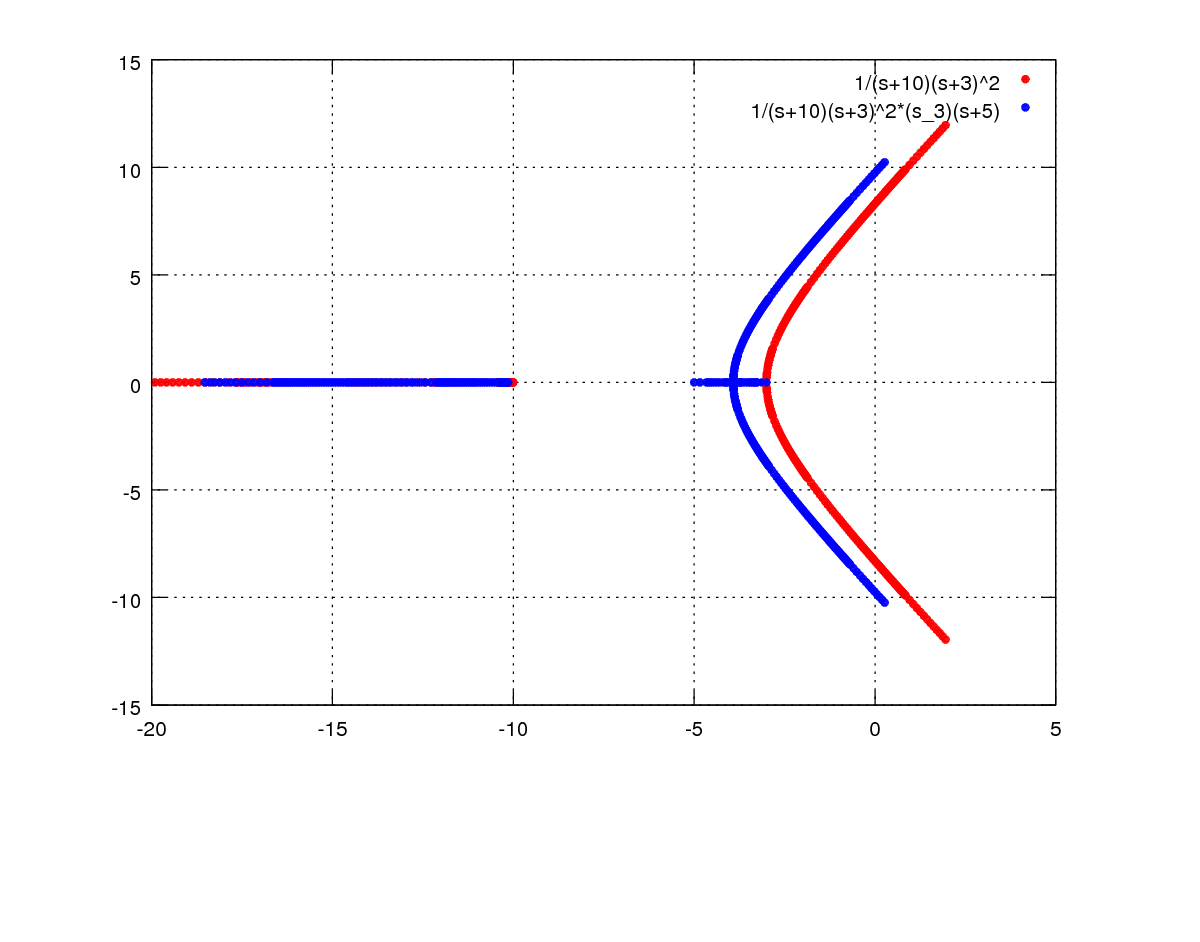
\includegraphics[width=10em]{image/lead.png}
\end{frame}
\begin{frame}
\frametitle{滞后校正}
\label{sec-3-2}

\begin{align*}
G(s) &=\frac{1}{(s+10)(s+3)^2}\\
G_c(s) &=\frac{10s+1}{100s+1}
\end{align*}

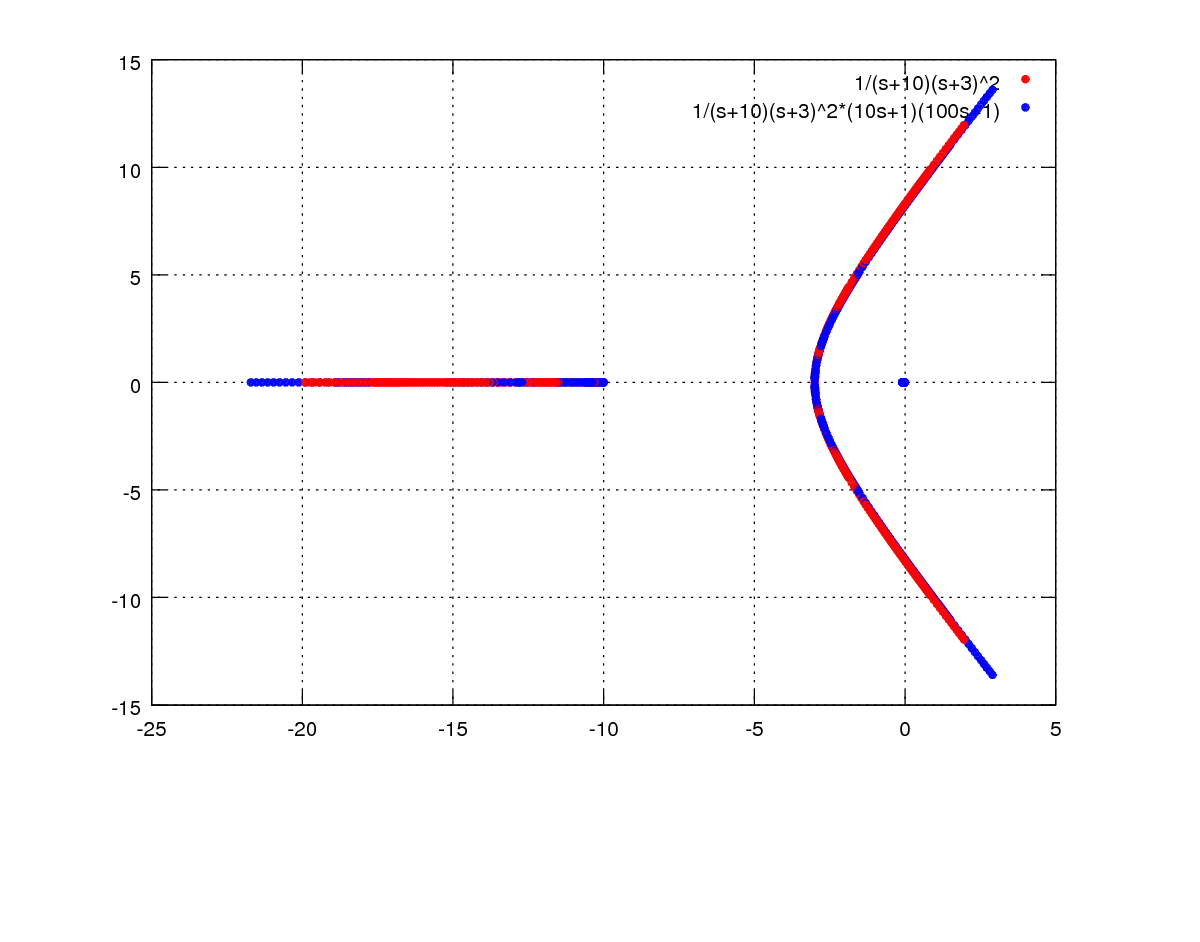
\includegraphics[width=10em]{image/lad.png}
\end{frame}

\end{document}
